\documentclass[xcolor=dvipsnames]{beamer}
\usepackage[utf8]{inputenc}
\usepackage{hyperref}
\usepackage[super]{nth} % for 1st, 2nd, etc...
\setbeamertemplate{caption}[numbered] %for figures numbering
\usepackage[export]{adjustbox} %for left and right
\usepackage{siunitx} % for degree symbol
\usepackage{hyperref}

\usetheme{CambridgeUS}

\definecolor{UBCblue}{rgb}{0.04706, 0.13725, 0.26667} % UBC Blue (primary)
\definecolor{UBCgrey}{rgb}{0, 0.46, 0.7} % UBC Grey (secondary)

\setbeamercolor{title}{bg=UBCblue,fg=white}
\setbeamercolor{frametitle}{bg=UBCblue, fg=white}
\setbeamercolor{palette primary}{bg=UBCblue,fg=white} %basso a destra
\setbeamercolor{palette secondary}{fg=UBCblue} %basso al centro
\setbeamercolor{palette tertiary}{bg=UBCgrey,fg=white} %basso e alto a sx 

\setbeamercolor{structure}{fg=UBCblue} % itemize, enumerate, etc
\setbeamercolor{section in toc}{fg=UBCblue} % TOC sections
\setbeamercolor{block title}{bg=UBCgrey!50,fg=black}
\setbeamercolor{block title example}{bg=UBCgrey!50,fg=black}

%------------------------------------------------------------
%This block of code defines the information to appear in the
%Title page
\title[Emotion Patterns in Music Playlists] %optional
{Emotion Patterns in Music Playlists}

%\subtitle{\nth{1} meeting}

\author[Sara, Mario] % (optional)
{Sara Giammusso\inst{1}\inst{2} \and Mario Guerriero \inst{1}\inst{2}}

\institute[EURECOM] % (optional)
{
 \inst{1}
 MSc student in Data Science Department, EURECOM, T\'el\'ecom ParisTech, France\\
  \inst{2}%
 MSc student in Department of Control and Computer Engineering, Politecnico di Torino, Italy
}


\date[2018 May 3] % (optional)
{Sixth Project meeting}


%End of title page configuration block
%-----------------------------------------------------------



%------------------------------------------------------------
%The next block of commands puts the table of contents at the 
%beginning of each section and highlights the current section:

\AtBeginSection[]
{
  \begin{frame}
    \frametitle{Table of Contents}
    \tableofcontents[currentsection]
  \end{frame}
}
%------------------------------------------------------------


\begin{document}

%The next statement creates the title page.
\frame{\titlepage}

%---------------------------------------------------------
%This block of code is for the table of contents after
%the title page
\begin{frame}
\frametitle{Table of Contents}
\tableofcontents
\end{frame}
%---------------------------------------------------------

\section{Introduction}
%Intoduction
\begin{frame}{Introduction}
\begin{block}{Previously On Sara\&Mario Project...}
We worked on feature engineering to see how we could improve our classifiers\\
\end{block}
Next steps:
\begin{itemize}
\item Make sure the POS tagger we are using is good
\item Make some experiments with other datasets
\item Keep working on feature engineering
\item Start looking at playlists
\end{itemize}
\end{frame}

%Model Description
\section{Last Week Summary}

\begin{frame}{POS Tagger Analysis}
\begin{itemize}
\item We are using spaCy's built-in POS tagger
\item There is no authoritative paper regarding its internal details
\item Our experiments suggest that it is good for our purpose
	\footnote{Please refer to the following Jupyter Notebook to know more about what we did on this topic: \url{https://github.com/sgiammy/emotion-patterns-in-music-playlists/blob/master/src/POS_tagger_verification.ipynb}}
	\begin{itemize}
	\item Each line is treated as a separate sentence
	\item The tagger is smart enough to recognize less common words and abbreviations (very common in songs)
	\end{itemize}
\end{itemize}
\end{frame}

\begin{frame}{More on Feature Engineering}
\begin{itemize}
\item We had built a big list of features in the past few weeks
\item We concluded that we do not need all of them (of course)
\item We got the best performances just by using a subset of 10 of them
	\footnote{For more information, please refer to \url{https://github.com/sgiammy/emotion-patterns-in-music-playlists/blob/master/src/Advanced_Feature_Engineering.ipynb}}
	\begin{itemize}
	\item WORD\_COUNT, ECHOISMS, SELFISH\_DEGREE, DUPLICATE\_LINES, IS\_TITLE\_IN\_LYRICS, VERB\_PRESENT, VERB\_PAST, VERB\_FUTURE, ADJ\_FREQUENCIES and PUNCT\_FREQUENCIES
	\end{itemize}
\end{itemize}
\end{frame}

\begin{frame}{MoodyLyrics + EmoInt}
\begin{itemize}
\item We are very limited by MoodyLyrics
	\footnote{https://github.com/sgiammy/emotion-patterns-in-music-playlists/blob/master/src/EmoInt.ipynb}
\item EmoInt is made of tweets classified according to four emotions: anger, fear, joy and sadness
	\begin{itemize}
	\item We have mapped anger to angry, joy to happy, sadness to sad and discarded fear
	\end{itemize}
\item We were able to increase our dataset by 2254 items
\item No good results at the end
\end{itemize}
\end{frame}

%Model Evaluation
\section{Feature Selection}

\begin{frame}{Two More Features}
We wanted to expand our model with two features
\begin{itemize}
\item Sentiment/Polarity
\item Subjectivity
\end{itemize}
To achieve this goal we used TextBlob\footnote{\url{http://textblob.readthedocs.io/en/dev/index.html}}
\begin{itemize}
\item Built on top of NLTK and Pattern
\item Makes use of Pattern's analyzer to generate polarity and subjectivity
\end{itemize}
At the end we will have 12 features (311 in reality, because the lyrics content vector is expanded)
\end{frame}

\begin{frame}{Obtained Results: ANN}
\begin{columns}
\column{0.5\textwidth}
\begin{figure}
	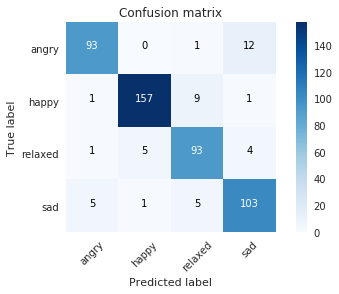
\includegraphics[scale=0.5,left]{./images/ann-ml-cm}
	\caption{90.84\% accuracy on MoodyLyrics}
\end{figure}

\column{0.5\textwidth}
\begin{figure}
	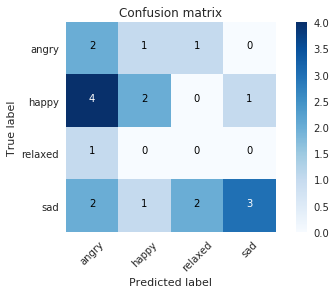
\includegraphics[scale=0.5,left]{./images/ann-extra-cm}
	\caption{50\% accuracy on extra test}
\end{figure}

\end{columns}
\end{frame}

\begin{frame}{Obtained Results: Logistic Regression\footnote{We experimented with several probabilistic classifiers and Logistic Regression was the one giving the best results}}
\begin{columns}
\column{0.5\textwidth}
\begin{figure}
	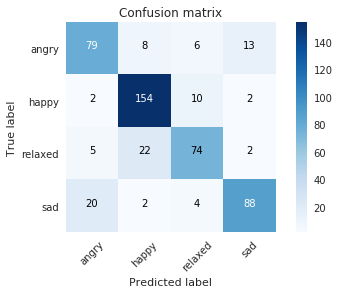
\includegraphics[scale=0.5,left]{./images/logreg-ml-cm}
	\caption{80\% accuracy on MoodyLyrics}
\end{figure}

\column{0.5\textwidth}
\begin{figure}
	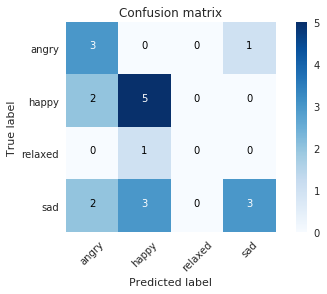
\includegraphics[scale=0.5,left]{./images/logreg-extra-cm}
	\caption{55\% accuracy on extra test}
\end{figure}

\end{columns}
\end{frame}

%Model Description
\section{Playlists Classification}

\begin{frame}{Which classification model?}
We considered different approaches
\begin{itemize}
\item Give each song in the playlist an emotion label and choose using a majority rule
\item Consider the text of all the songs in a playlist as belonging to a single song and classify it
\item Compute an "emotion vector" for each song and average all of those vectors over the playlist
	\footnote{Remember the sliders approach? We got inspired from this}
	\begin{itemize}
	\item This is the one which makes more sense to us
	\item It produces 4 playlist features (one per emotion) you may want to use in your recommendation system
	\end{itemize}
\end{itemize}
\end{frame}

\begin{frame}{Our Results\footnote{We will try to keep this notebook updated with all future statistics: \url{https://github.com/sgiammy/emotion-patterns-in-music-playlists/blob/master/src/Playlist_Classification_Stats.ipynb}}}
\begin{columns}
\column{0.5\textwidth}
\begin{figure}
	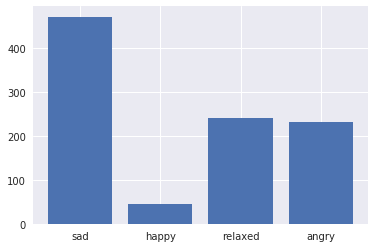
\includegraphics[scale=0.45,left]{./images/playlist-emotion-distribution-ann}
	\caption{Playlists emotion distribution with ANN}
\end{figure}

\column{0.5\textwidth}
\begin{figure}
	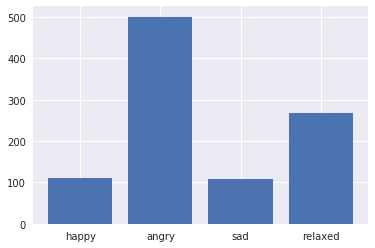
\includegraphics[scale=0.45,left]{./images/playlist-emotion-distribution-logreg}
	\caption{Playlists emotion distribution with Logistic Regression}
\end{figure}
\end{columns}
\end{frame}


%Conclusions
\section{Conclusion}

\begin{frame}{What's next?}
\begin{itemize}
\item We can't evaluate our results
\item Could you please test them inside your recommendation system?
\item Can we start writing our report? (if yes, any hint?)
\item ...
\end{itemize}
\end{frame}

%---------------------------------------------------------

\end{document}
